\section{Introduction}

As one of the most popular research topics in the field of natural language processing, sentiment analysis tasks have been widely researched and applied in various fields such as academic research and product review mining, social opinion analysis, content-based recommendation, and so on.
People's experience and sentimental expression of objective things are often subjective and diverse, either by giving direct subjective statements of opinions, or by using facts or rhetorical hints to ideas, that is, by using sentences that do not contain obvious sentimental cues can also express a subjective sentiment. In connection with real life, people actually use a lot of implicit expressions to convey their feelings. There are examples as shown in the Fig~\ref{fig:Example}~.

\begin{figure}[h]
    \centering
    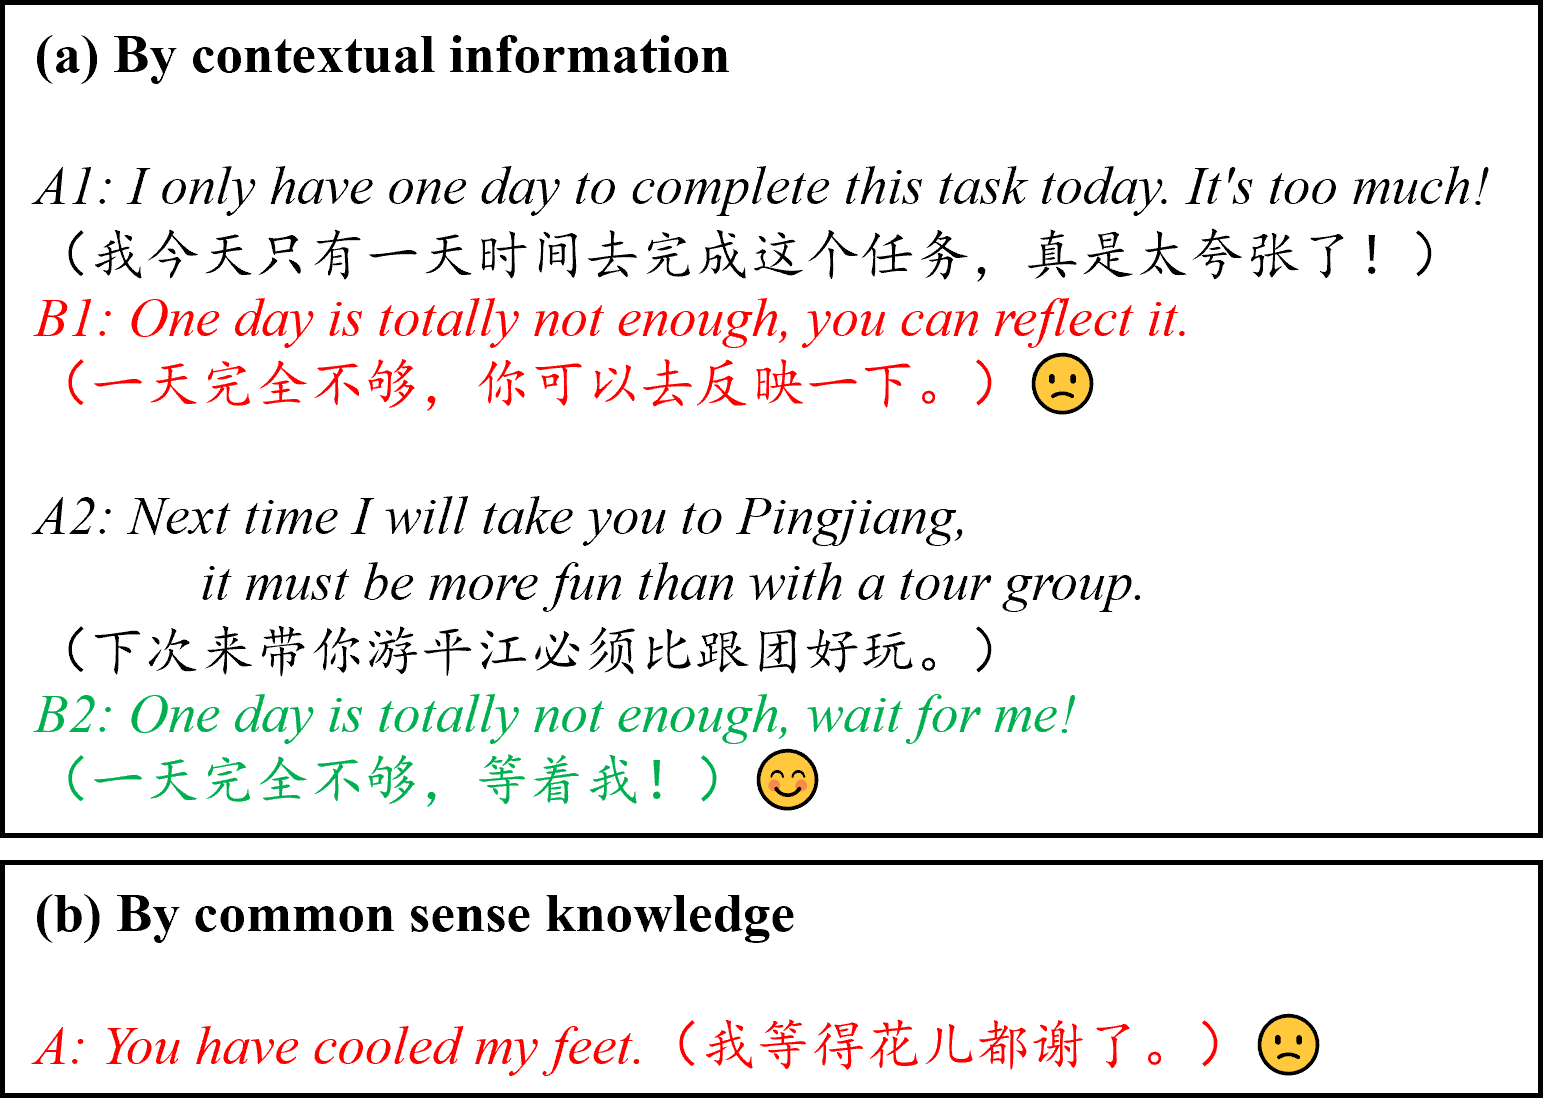
\includegraphics[width=0.5\linewidth]{submissions/knowledge-sentiment-analysis/2.png}
    \caption{Sentences with different contexts or based on external common sense knowledge can express different sentiments. Expressions carrying positive (smiling face) or negative (crying face) sentiments are highlighted in color. }
    \label{fig:Example}
\end{figure}

Both of the above examples do not contain obvious sentimental cues, but they invariably convey the speaker's sentimental disposition.
Sentiment expressed implicitly rather than using words with sentimental colors are called ``implicit sentiment"\cite{PanDongXing2020}.
For the task of text sentiment analysis in natural language processing, sentiment texts can be classified into explicit sentiment analysis and implicit sentiment analysis according to whether they contain obvious sentiment words in their expressions\cite{liu2020sentiment}.
Statistical analysis of related studies\cite{jian2016constitution,chen2016implicit,liao2019identification} shows that implicit sentiment sentences are more common in Chinese, accounting for about 20\% to 30\% of all sentences with sentiment tendencies.
Explicit sentiment sentences contain explicit sentiment vocabulary with strong semantic feature information, which can help sentiment analysis models accurately predict the sentiment tendency in sentences, and therefore many research results have emerged in the field of explicit sentiment analysis.
On the contrary, implicit sentiment expressions do not have such characteristics, and the expressions are more obscure. For the current task of Chinese implicit sentiment analysis, there are two main critical problems faced:


Chinese implicit sentiment analysis requires the introduction of contextual information. Example (a) is an instance of the same expression expressing different sentimental tendencies in different contexts. The speaker conveys two opposite sentimental tendencies, negative (B1) and positive (B2), through the similar emotional expression ``One day is totally not enough" according to the content received above. Thus, implicit sentiment analysis suffers from the problem that the sentiment expression itself does not provide enough information, and contextual information needs to be introduced.

Chinese implicit sentiment analysis lacks the support of external knowledge. Example (b) is a declarative sentence using metaphorical rhetoric. Although it does not contain any sentimental cues such as ``anxious", etc., it effectively conveys the sentiment that the speaker has been waiting for a long time and is somewhat dissatisfied. Therefore, combined with human understanding of implicit sentimental expression, it is necessary to introduce an understanding of external common sense knowledge to support the discernment of implicit sentimental tendencies.

In order to address typical problems in Chinese implicit sentiment analysis tasks like those two listed above, we propose a sentiment analysis method in this paper that integrates contextual information and external common sense knowledge for implicit sentiment analysis.

The main contributions of this paper can be summarized as follows:

\begin{enumerate}

\item We propose a retrieval method to extract valid sentiment triads from a knowledge base and build an adaptive fusion of external common sense knowledge embedding layers to extend the semantic information of implicit sentiment expressions. Such improvements significantly facilitate the mining of implicit sentiment expressions hidden in ambiguous language fragments without sentiment words as clues.

\item Multipolar orthogonal attention mechanism is used to learn embedding representations for implicit sentiment expressions, and an attention layer that incorporates context is introduced to mine and combine valid information in the context. This effectively retains the differences between attention representations and thus contributes to distinguishing subtle differences between sentiment polarities.

\item The common sense knowledge information provided by the external knowledge base is fused with the contextual representation and the semantic information of the sentiment expression itself to achieve an effective extension of the implicit sentiment sentence representation and to perform sentiment label prediction. The experimental results show that our model obtains more satisfactory performance than the baseline models.

\end{enumerate} 